\documentclass[titlepage, letterpaper, fleqn]{article}
\usepackage[utf8]{inputenc}
\usepackage{fancyhdr} % fancy headers, of course!
\usepackage{amsmath} % what do you think?
\usepackage{amsthm} % theorems!
\usepackage{extramarks} % more cute things
\usepackage{enumitem} % i'm not sure...
\usepackage{multicol} % multicolumn...?
\usepackage{amssymb} % more symbols
\usepackage{MnSymbol} % moar symbols?
\usepackage{booktabs} % cool looking tables
\usepackage{tikz} %venn and shizzle
\usepackage{tikz-qtree-compat} %tableaux
\usepackage{lipsum} %lorem ipsum dolor sit amet f u
\usepackage{mathrsfs} %math script for calligraphic scripting, I GUESS

\topmargin=-0.45in
\evensidemargin=0in
\oddsidemargin=0in
\textwidth=6.5in
\textheight=9.0in
\headsep=0.25in


%
% You should change this things~
%

\newcommand{\mahteacher}{Dr. Viacheslav Kalashnikov}
\newcommand{\mahclass}{Applied Mathematics}
\newcommand{\mahtitle}{Topic IV - Activity 23}
\newcommand{\mahdate}{November 16, 2016}
\newcommand{\spacepls}{\vspace{5mm}}
\newcommand{\until}{\mathscr{U}}
\renewcommand\qedsymbol{\(\blacksquare\)}

%
% Header markings
%

\pagestyle{fancy}
\lhead{1170065 - Xavier Sánchez}
\chead{}
\rhead{}
\lfoot{}
\rfoot{}


\renewcommand\headrulewidth{0.4pt}
\renewcommand\footrulewidth{0.4pt}

\setlength\parindent{0pt}


%
% Create Problem Sections (stolen directly from jdavis/latex-homework-template @ github!)
%

\newcommand{\enterProblemHeader}[1]{
\nobreak\extramarks{}{Problem \arabic{#1} continued on next page\ldots}\nobreak{}
\nobreak\extramarks{Problem \arabic{#1} (continued)}{Problem \arabic{#1} continued on next page\ldots}\nobreak{}
}

\newcommand{\exitProblemHeader}[1]{
\nobreak\extramarks{Problem \arabic{#1} (continued)}{Problem \arabic{#1} continued on next page\ldots}\nobreak{}
\stepcounter{#1}
\nobreak\extramarks{Problem \arabic{#1}}{}\nobreak{}
}

\setcounter{secnumdepth}{0}
\newcounter{partCounter}
\newcounter{homeworkProblemCounter}
\setcounter{homeworkProblemCounter}{1}
\nobreak\extramarks{Exercise \arabic{homeworkProblemCounter}}{}\nobreak{}

%Solution Environment
\newenvironment{solution}
{\renewcommand\qedsymbol{$\square$}\begin{proof}[Solution]}
{\end{proof}}

% Alias for the Solution section header
%\newcommand{\solution}{\textbf{\Large Solution}}

%Alias for the new step section
\newcommand{\steppy}[1]{\textbf{\large #1}}

%
% Homework Problem Environment
%
% This environment takes an optional argument. When given, it will adjust the
% problem counter. This is useful for when the problems given for your
% assignment aren't sequential. See the last 3 problems of this template for an
% example.
%
\newenvironment{homeworkProblem}[1][-1]{
\ifnum#1>0
\setcounter{homeworkProblemCounter}{#1}
\fi
\section{Exercise \arabic{homeworkProblemCounter}}
\setcounter{partCounter}{1}
\enterProblemHeader{homeworkProblemCounter}
}{
\exitProblemHeader{homeworkProblemCounter}
}

%
% My actual info
%

\title{
\vspace{1in}
\textbf{Tecnológico de Monterrey} \\
\vspace{0.5in}
\textmd{\mahclass} \\
\large{\textit{\mahteacher}} \\
\vspace{0.5in}
\textsc{\mahtitle}\\
\textsc{Analysis of Variance (ANOVA)}\\
\textsc{4.6.1}\\
\author{01170065  - MIT \\
Xavier Fernando Cuauhtémoc Sánchez Díaz \\
\texttt{mail@gmail.com}}
\date{\mahdate}
}

\begin{document}

\begin{titlepage}
\maketitle
\end{titlepage}

%
% Actual document starts here~
%

\section{Exercise 4.6.1}

{\large A purification process for a chemical involves passing it, in solution, through a resin on which impurities are adsorbed.
A chemical engineer wishing to test the efficiency of 3 different resins took a chemical solution and broke it into 15 batches.
She tested each resin 5 times and then measured the concentration of impurities after passing through the resins. Her data were as follows:}

\begin{table}[h!]
\centering
\begin{tabular}{@{}ccc@{}}
\toprule
Resin I & Resin II & Resin III \\ \midrule
0.046 & 0.038 & 0.031 \\
0.025 & 0.035 & 0.042 \\
0.014 & 0.031 & 0.020 \\
0.017 & 0.022 & 0.018 \\
0.043 & 0.012 & 0.039 \\ \bottomrule
\end{tabular}
\caption{Concentration of Impurities}
\label{tab4.6.1}
\end{table}

{\large Test the hypothesis that there is no difference in the efficiency of the resins.}

\begin{solution}
Let $H_0$ be the hypothesis that $\mu_0 = \mu_1 = \mu_2$,
versus $H_1$ that not all the means are equal.

First we start by computing the between samples sum of squares using $SS_b = n\sum\limits_{i=1}^m(X_{i.} - X_{..})^2$

For that, we need the mean of each sample: $X_{1.} = 0.029, X_{2.} = 0.0276, X_{3.} = 0.03$, and also  the estimator of $\mu, X_{..} = \dfrac{\sum\limits_{i=1}^m X_{i.}}{m} = 0.028866667$.

We can now calculate $SS_b = 0.000014533$.

We now calculate the sum of squares $SS = \sum\limits_{i=1}^n\sum\limits_{j=1}^m$, where $n$ is the number of samples (3) and $m$ is the number of measurements in each sample.

Replacing the values, we have:
\[SS = \sum\limits_{i=1}^3\sum\limits_{j=1}^5 = 0.014303\]

We now need to compute SSW using the equation $SS_W = SS - nmX_{..}^2 - SS_b$ which yields 0.0017892.

This number is later used in the test statistic $TS = \dfrac{SS_b / (m-1)}{SS_W/(nm-m)} = 0.0487368$.

After that, the test statistic is checked against the $F$ value from the table, specifically $F_{m-1,nm-m,\alpha} = F_{2,12,0.05} = 3.89$.

Since $TS < F_{2,12,0.05}$, we have not enough evidence to reject $H_0$.

\begin{figure}[htbp]
	\centering
	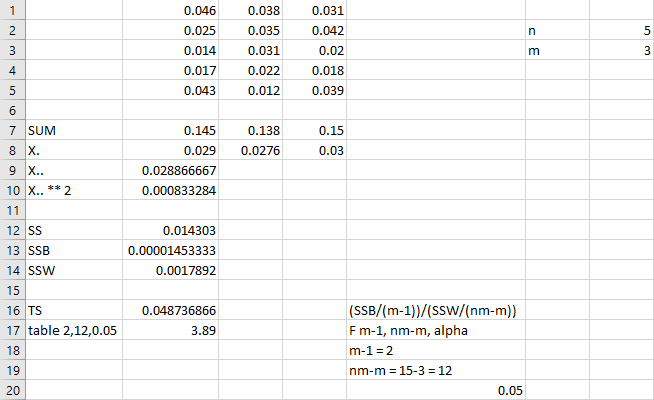
\includegraphics[width=0.98\textwidth]{img_4_6_1}
	\caption{Screen capture of the software used for computations}
	\label{fig:4.6.1}
\end{figure}

Software was used for most of the computations, as can be seen in Fig. \ref{fig:4.6.1}
\end{solution}

\end{document}